\documentclass[%
    %handout
]{beamer}
\usepackage{graphicx} % For including single page pdfs
\usepackage{bm}       % bold math
\usepackage{pgffor}   % for loop
\usepackage{tikz}
\usepackage{multimedia}
\usepackage{layouts}
\usepackage{hyperref}
\usepackage{cambridge_lecture}
\usepackage{mathtools}
\newtheorem*{theorem*}{Theorem}


\title{Derived parameters with specified distributions}
\subtitle{Maximum entropy prior choices}
\author[Handley] % (optional, for multiple authors)
{Will Handley\\ \small{wh260@cam.ac.uk}}
\institute[University of Cambridge] % (optional)
{%
Astrophysics Group \\
Cavendish Laboratory \\
University of Cambridge
}
\date{16\textsuperscript{th} May 2018}

\usepackage{calculator}

\newcommand{\cols}[3][0.5]{%
    \SUBTRACT{1.}{#1}{\wdthb}
    \begin{columns}
        \begin{column}{#1\textwidth}
            #2
        \end{column}
        \begin{column}{\wdthb\textwidth}
            #3
        \end{column}
    \end{columns}
}

\newcommand{\figname}{}
\newenvironment{figright}[2][0.5]{%
    \renewcommand{\figname}{#2}
    \SUBTRACT{1.}{#1}{\wdthb}
    \begin{columns}
        \begin{column}{#1\textwidth}
        }{%
        \end{column}
        \begin{column}{\wdthb\textwidth}
            \includegraphics[width=\textwidth]{\figname}
        \end{column}
    \end{columns}
}

\newcommand{\dfigname}{}
\newenvironment{dfigright}[3][0.5]{%
    \renewcommand{\figname}{#2}
    \renewcommand{\dfigname}{#3}
    \SUBTRACT{1.}{#1}{\wdthb}
    \begin{columns}
        \begin{column}{#1\textwidth}
        }{%
        \end{column}
        \begin{column}{\wdthb\textwidth}
            \includegraphics[width=\textwidth]{\figname}
            \includegraphics[width=\textwidth]{\dfigname}
        \end{column}
    \end{columns}
}



\newenvironment{figleft}[2][0.5]{%
    \SUBTRACT{1.}{#1}{\wdthb}
    \begin{columns}
        \begin{column}{#1\textwidth}
            \includegraphics[width=\textwidth]{#2}
        \end{column}
        \begin{column}{\wdthb\textwidth}
        }{%
        \end{column}
    \end{columns}
}

\newenvironment{dfigleft}[3][0.5]{%
    \SUBTRACT{1.}{#1}{\wdthb}
    \begin{columns}
        \begin{column}{#1\textwidth}
            \includegraphics[width=\textwidth]{#2}
            \includegraphics[width=\textwidth]{#3}
        \end{column}
        \begin{column}{\wdthb\textwidth}
        }{%
        \end{column}
    \end{columns}
}


\newcounter{numimages}

\newenvironment{multifig}[1]{%
    \begin{frame}
        \pdfximage{#1}%
        \setcounter{numimages}{\the\pdflastximagepages}
        \addtocounter{numimages}{-1}

        \begin{tikzpicture}[remember picture, overlay]
            \foreach \pagenum in {1,...,\thenumimages} {%
                \node<handout:0|beamer:\pagenum>[anchor=center] at (current page.center) {
                \includegraphics[width=\textwidth,page=\pagenum]{#1}}; 
            }
            \addtocounter{numimages}{1}
            \node<handout:1|beamer:\thenumimages>[anchor=center] at (current page.center) {
            \includegraphics[width=\textwidth,page=\thenumimages]{#1}}; 
        \end{tikzpicture}
    }{%
    \end{frame}
}


\begin{document}

\begin{frame}
    \titlepage{}
\end{frame}

\begin{frame}
    \frametitle{Bayesian inference}
    \begin{columns}
        \begin{column}{0.6\textwidth}
            \begin{itemize}
                \item Model parameters $x$ describing data $D$:
                    \begin{align}
                        P(x|D) &= \frac{P(D|x) P(x)}{P(D)}
                        \nonumber\\
                        \text{Posterior} &= 
                        \frac{\text{Likelihood}\times \text{Prior}}{\text{Evidence}}
                        \nonumber
                    \end{align}
                \item Need Prior distribution $P(x)$
                \item Chosen to reflect initial knowledge, without data
                \item Harder to do with modern inference techniques:
                    \begin{itemize}
                        \item Non-parametric (model-independent) reconstructions
                        \item Hierarchical models
                    \end{itemize}
            \end{itemize}
        \end{column}
        \begin{column}{0.4\textwidth}
            
\newcommand{\movablecross}[1]{%
    \draw[->](#1) -- ++(0:\croslen);
    \draw[->](#1) -- ++(90:\croslen);
    \draw[->](#1) -- ++(180:\croslen);
    \draw[->](#1) -- ++(270:\croslen);
    \fill[red!70!black] (#1) circle (2pt);
}

\newcommand{\movablevert}[1]{%
    \draw[->](#1) -- ++(90:\croslen);
    \draw[->](#1) -- ++(270:\croslen);
    \fill[red!70!black] (#1) circle (2pt);
}

\begin{tikzpicture}
    % width of axes
    % length of crosses
    \def\croslen{0.1\textwidth}


    % Draw axes
    \draw [<->,thick] (0,0.67\textwidth) node (yaxis) [above] {$y$}
    |- (\textwidth,0) node (xaxis) [below] {$x$};

    % Draw the line joining start and end
    \coordinate (mn) at (0.1\textwidth,0.3\textwidth);
    \coordinate (start) at (0.2\textwidth,0.6\textwidth);
    \coordinate (mid) at (0.5\textwidth,0.2\textwidth);
    \coordinate (end) at (0.6\textwidth,0.5\textwidth);
    \coordinate (mx) at (0.9\textwidth,0.4\textwidth);
    \draw (mn) node[below right]    {$(x_1,y_1)$};
    \draw (start) node[above right]     {$(x_2,y_2)$};
    \draw (mid) node[below right] {$(x_3,y_3)$};
    \draw (end) node[above right] {$(x_4,y_4)$};
    \draw (mx) node[below left]  {$(x_N,y_N)$};
    \movablevert{mn};
    \movablevert{mx};
    \movablecross{start};
    \movablecross{mid};
    \movablecross{end};

    \draw (mn) -- (start) -- (mid) -- (end) -- (mx);



\end{tikzpicture}


            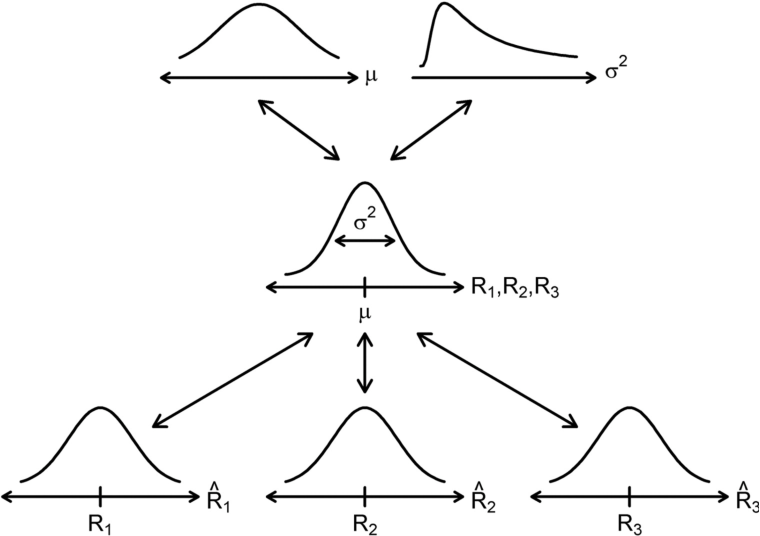
\includegraphics[width=0.95\textwidth]{figures/hierarchical.pdf}
        \end{column}
    \end{columns}
\end{frame}

\begin{frame}
    \frametitle{Prior construction}
    \framesubtitle{The principle of maximum entropy}
    \begin{itemize}
        \item We may wish to construct a prior ``assuming the least information''
        \item One way to quantify this is using the Shannon entropy:
            \begin{equation}
                H(\Omega) 
                = \sum_{E\in \Omega} P(E) \log \frac{1}{P(E)}
                \nonumber
            \end{equation}
        \item Shannon information 
            \begin{equation}
                \mathcal{I}(E) = \log \frac{1}{P(E)},
                \qquad
                H = \left\langle\log \mathcal{I}(E)\right\rangle_{E\in \Omega}
                \nonumber
            \end{equation}
        \item We construct priors by minimising $H$, subject to knowledge constraints
    \end{itemize}
\end{frame}

\begin{frame}
    \frametitle{Maximum entropy prior examples}
    \begin{itemize}
        \item Known mean $\mu$ and variance $\sigma$ $\Rightarrow$ Gaussian:
            \begin{equation}
                P(x) = \tfrac{1}{\sqrt{2\pi}\sigma}\exp\left[-\tfrac{{(x-\mu)}^2}{2\sigma^2}\right]
                \nonumber
            \end{equation}
        \item Known mean $x_0$ and positive $x>0$ $\Rightarrow$ Exponential:
            \begin{equation}
                P(x) = \tfrac{1}{x_0}\exp\left[-x/x_0\right]
                \nonumber
            \end{equation}
        \item Positive $x>0$ $\Rightarrow$ Logarithmic (improper):
            \begin{equation}
                P(x) \propto 1/x
                \nonumber
            \end{equation}
        \item Nothing  $\Rightarrow$ Uniform (improper):
            \begin{equation}
                P(x) \propto 1
                \nonumber
            \end{equation}
    \end{itemize}
\end{frame}

\begin{frame}
    \frametitle{The importance of plotting priors}
    \framesubtitle{VSA cosmological parameters (astro-ph:0212497)}

    \begin{columns}
        \begin{column}{0.5\textwidth}
        \begin{itemize}
            \item<1-> Consider constraint on Hubble parameter $h$ $(H_0 = 100h\frac{\mathrm{kms}^{-1}}{\mathrm{Mpc}})$
            \item<3-> $h$-constraint {\em gets worse\/} with data
            \item<3-> Lesson: It is essential to plot priors and posteriors together.
            \item<3-> Particularly relevent for new data with weak constraints (e.g. EoR)
        \end{itemize}
        \end{column}
        \begin{column}{0.5\textwidth}
            \includegraphics<1>[width=\textwidth]{figures/vsa_prior}
            \includegraphics<2->[width=\textwidth]{figures/vsa_posterior}
        \end{column}
    \end{columns}
\end{frame}

\begin{frame}
    \frametitle{Non-parametric reconstructions}
    \framesubtitle{Example: cosmic reionisation history from CMB (Millea \& Bouchet 1804.08476)}
    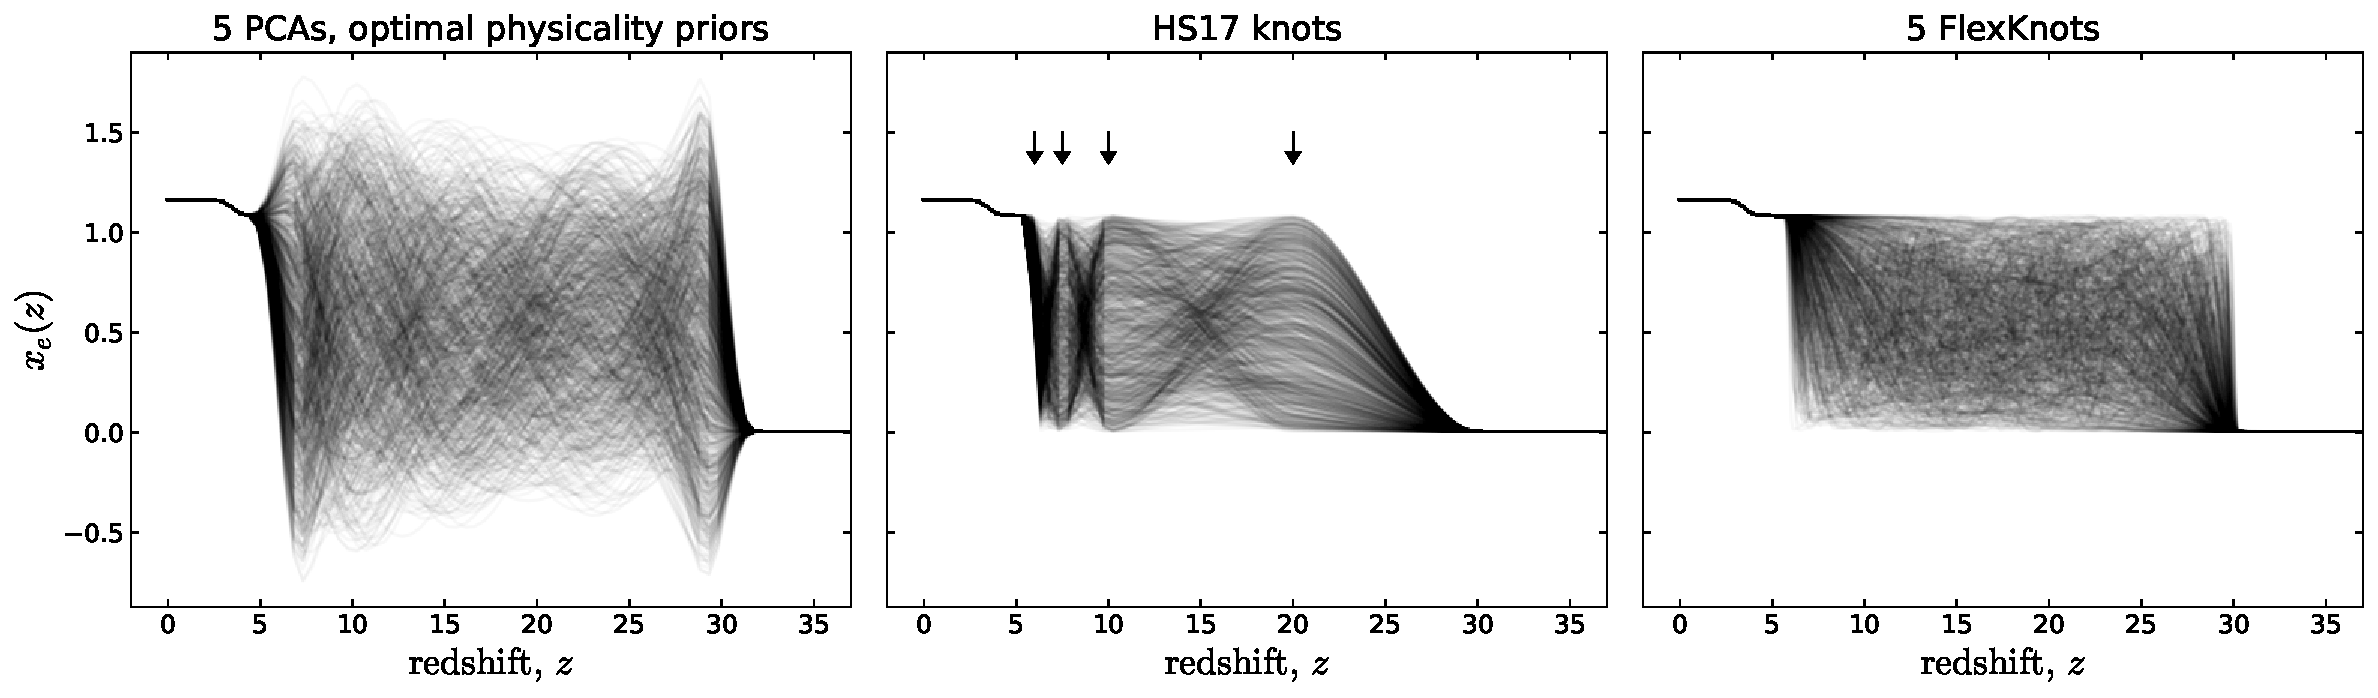
\includegraphics[width=\textwidth]{figures/reio_hists_prior}
    \begin{itemize}
        \item Aim to reconstruct reionisation history $x_\mathrm{e}(z)$ from Planck data 
        \item Model-independent/non-parametric
        \item Optical depth $\tau = \int \frac{n_\mathrm{H}(z){(1+z)}^2}{H(z)}x_\mathrm{e}(z) dz $
        \item Reconstruction introduces non-trivial prior on derived parameter $\tau$
    \end{itemize}
\end{frame}

\begin{frame}
    \frametitle{Tau prior and posterior}
    \framesubtitle{Example: cosmic reionisation history from CMB (Millea \& Bouchet 1804.08476)}
    \centerline{%
        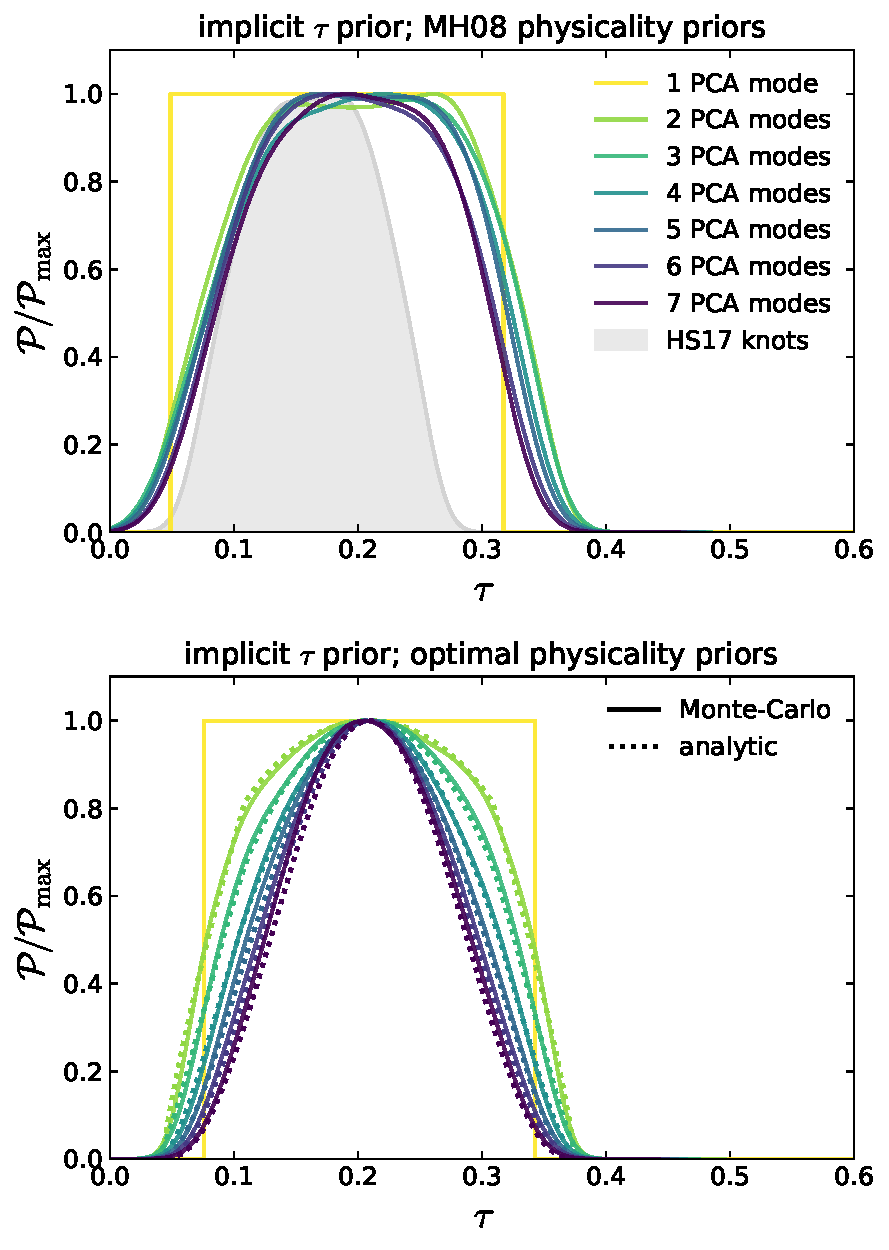
\includegraphics[width=0.45\textwidth]{figures/implicit_tau_priors}
        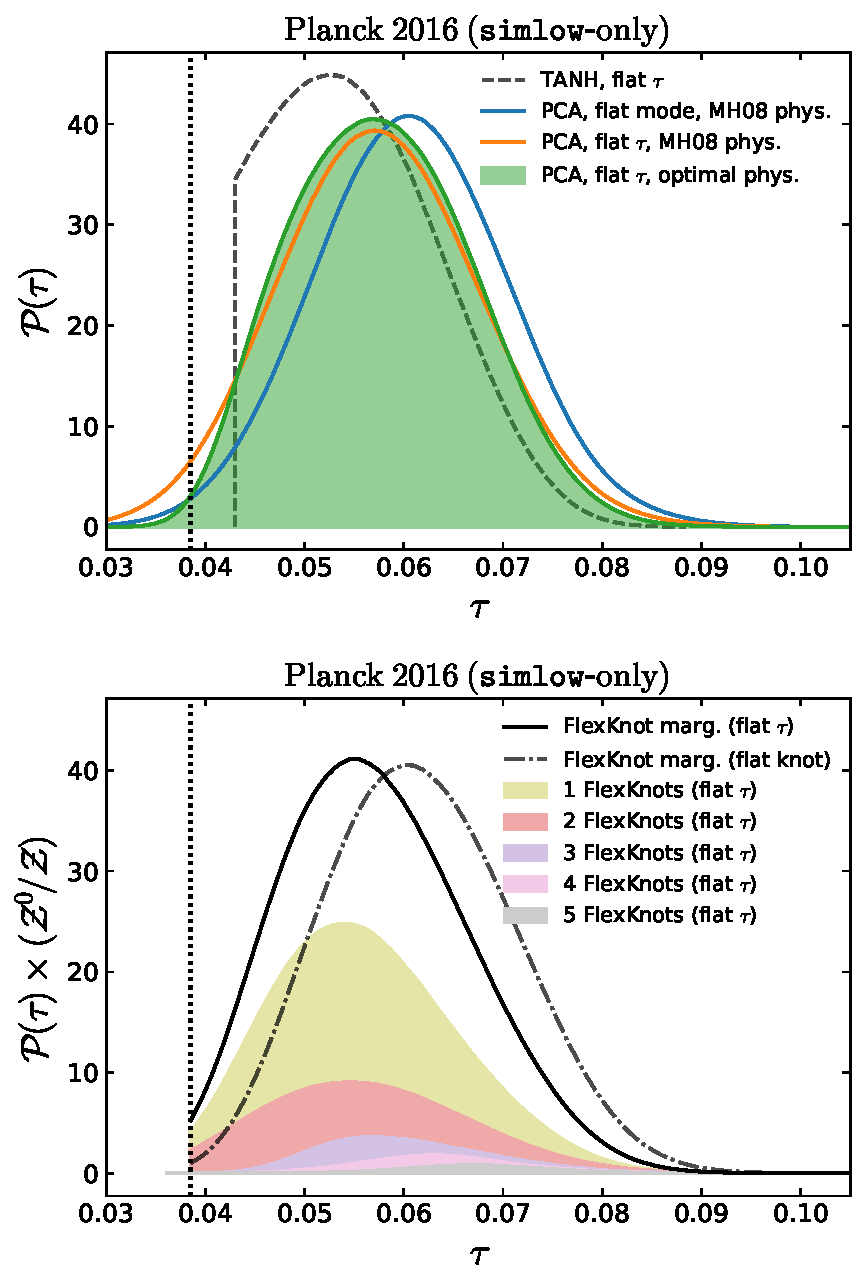
\includegraphics[width=0.45\textwidth]{figures/data_simlow}
    }
\end{frame}

\begin{frame}
    \frametitle{Reionisation posterior}
    \framesubtitle{Example: cosmic reionisation history from CMB (Millea \& Bouchet 1804.08476)}
    \centerline{%
        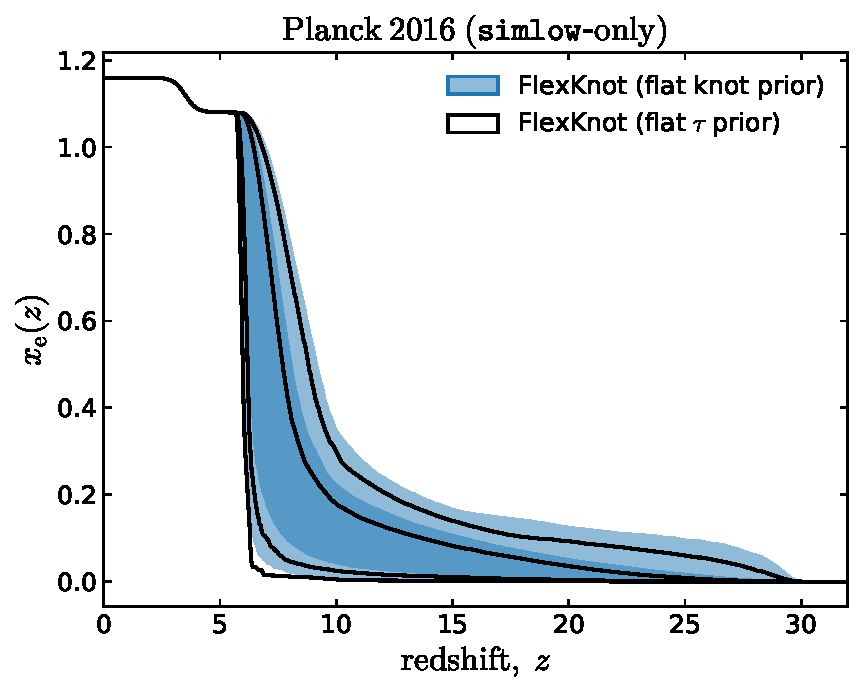
\includegraphics[width=0.8\textwidth]{figures/reio_hists_simlow}
    }
\end{frame}

\begin{frame}
    \frametitle{Derived parameter priors}
    \framesubtitle{Simplified example}
    \begin{columns}
        \begin{column}{0.5\textwidth}
        \begin{itemize}
            \item Uniform distribution $q(a,b)$
            \item $\Rightarrow$ triangular distribution on $a+b$.
            \item Remove this effect by dividing out this distribution:
                \begin{equation}
                    p(a,b) = \frac{q(a,b)}{q(a+b)}
                    \nonumber
                \end{equation}
            %\item<2-> $p(a,b)$ is adjusted to counterbalance tails of $q(a+b)$.
        \end{itemize}
        \end{column}
        \begin{column}{0.5\textwidth}
            \includegraphics<1>[width=\textwidth]{figures/q}
            \includegraphics<2->[width=\textwidth]{figures/p}
        \end{column}
    \end{columns}
\end{frame}

\begin{frame}
\frametitle{General result: This is maximum entropy}
\framesubtitle{Handley \& Millea 1804.08143}
\begin{theorem*}
    If one has a distribution on parameters $x$ with probability density function $q(x)$ along with a derived parameter $f$ defined by a function $f=f(x)$, then the maximum entropy distribution $p(x)$ relative to $q(x)$ satisfying the constraint that $f$ is distributed with probability density function to $r(f)$ is:
\begin{equation}
    p(x)  = \frac{q(x)r(f(x))}{P(f(x)|q)},\label{eqn:final_answer}
    \nonumber
\end{equation}
where $P(f|q)$ is the probability density for the distribution induced by $q$ on $f=f(x)$.
\end{theorem*}
\end{frame}

\begin{frame}
    \frametitle{Derived parameter priors}
    \framesubtitle{Neutrino example}
	\begin{figright}{figures/neutrino_masses}
        \begin{itemize}
            \item Initial spherical log-gaussian $q$
            \item $\Rightarrow$ non-trivial shifted distribution on mass sum $m_1+m_2+m_3$
            \item Apply maxent prior forcing this distribution back to center
            \item Creates heavy tail previously ruled out by $q$.
        \end{itemize}
	\end{figright}
\end{frame}

%\begin{frame}
%    \frametitle{<++>}
%    \framesubtitle{<++>}
%\end{frame}

%\begin{frame}
%    \frametitle{<++>}
%    \framesubtitle{<++>}
%
%	\begin{figright}{<++>}
%	\end{figright}
% 
%\end{frame}


\begin{frame}[label=further_reading]
    \frametitle{Further reading}
    \centerline{%
        \hfill{}
        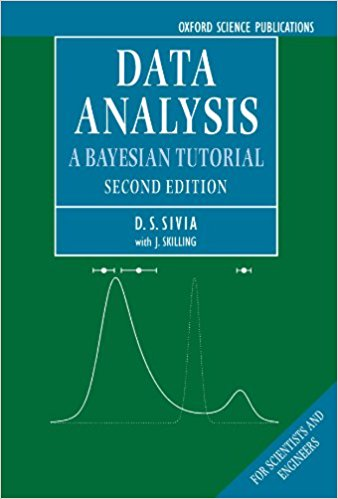
\includegraphics[height=0.7\textheight]{./figures/sivia_skilling.jpg}
        \hfill{}
        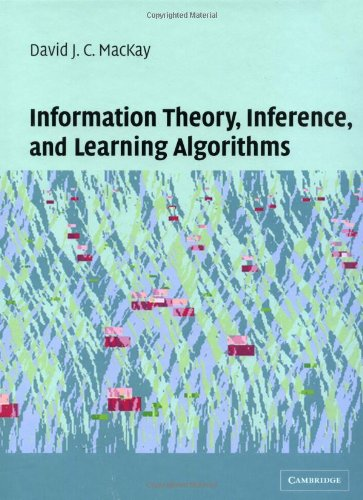
\includegraphics[height=0.7\textheight]{./figures/mackay.jpg}
        \hfill{}
    }
    \begin{itemize}
        \item Data analysis: A Bayesian Tutorial (Sivia \& Skilling)
        \item Information Theory, Inference and Learning Algorithms (Mackay)
    \end{itemize}
\end{frame}



\end{document}
